\documentclass[12pt,twocolumn]{article}
\usepackage[margin=1.5cm]{geometry}
\usepackage{amsmath}
\usepackage{graphicx}
\usepackage{hyperref}
\usepackage{sectsty}
\title{Midterm 1 Solutions}
\author{Prof. Jordan C. Hanson}
\sectionfont{\fontsize{12}{15}\selectfont}

\begin{document}
\maketitle
\small

\section{Unit 0: Electrostatics I and II}

\noindent
\begin{enumerate}
\item (a) What is the force on the charge located at $x=8.00$ cm in Fig. \ref{fig:e-field_1}(a) given that $q=1.00$ $\mu$C? (b) Find the total electric field at $x=11.00$ cm in Fig. \ref{fig:e-field_1}(b). \\ \\
\textit{(a) 12.6 N, using Coulomb's Law for each chare. (b) $4.07 \times 10^{7}$ N/C, using the Coulomb field for point charges.}
\begin{figure}
\centering
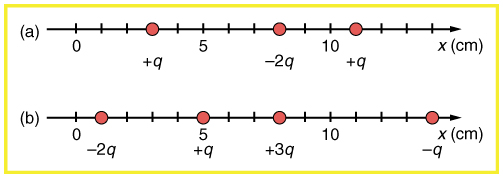
\includegraphics[width=0.49\textwidth]{e-field_1.jpeg}
\caption{\label{fig:e-field_1} Linear arrangement of charges.}
\end{figure}
\item Determine the direction of the force on $q$ in Fig. \ref{fig:e-field_2}, given that $q_a=q_b=+7.50$ $\mu$C and $q_c = q_d = -7.50$ $\mu$C. (b) Calculate the force on the charge $q$, given that the square is 10.0 cm on a side and $q=2.00$ $\mu$C.
\begin{figure}[hb]
\centering
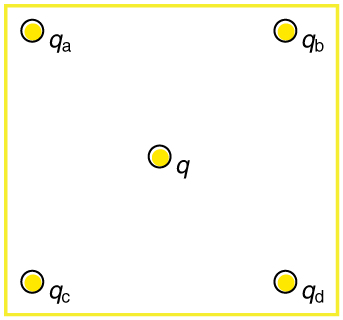
\includegraphics[width=0.25\textwidth]{e-field_2.jpeg}
\caption{\label{fig:e-field_2} 2D arrangement of charges.}
\end{figure}
\textit{(a) Down, by symmetry. (b) We can show that the total force is $8 k q q_a/a^2$, in the downward direction.  Only the y-components survive, and the angle between the force and y-component of the force is 45 degrees (square).  If the side length is $a$, the distance between corners and center is $a/\sqrt{2}$.  The result is 108 N.}
\item An evacuated tube uses an accelerating voltage of 40 kV to accelerate electrons to hit a copper plate and produce x rays. Non-relativistically, what would be the maximum speed of these electrons? \\ \\
\textit{This problem is about energy conservation.  Equate the potential energy (voltage times charge) with the kinetic energy to find velocity.  The result is $11.8 \times 10^7$ m/s.  This is about 40 percent the speed of light.}
\item The electric field strength between two parallel conducting plates separated by 4.00 cm is $7.50 \times 10^4$ V m$^{-1}$. (a) What is $\Delta V$ between the plates? (b) The plate with the lowest potential is taken to be at zero volts. What is the potential 1.00 cm from that plate (and 3.00 cm from the other)? (c) The voltage across a membrane forming a cell wall is 80.0 mV and the membrane is 9.00 nm thick. What is the electric field strength?\footnote{The value is surprisingly large, but correct.} \\ \\
\textit{(a) 1.5 kV. (b) 375 V. (c) $9\times 10^6$ V/m.}
\item A doubly charged ion is accelerated to an energy of 32.0 keV by the electric field between two parallel conducting plates separated by 2.00 cm. What is the electric field strength between the plates? \\ \\
\textit{8 kV/cm, or $8\times 10^5$ V/m.}
\item In one of the classic nuclear physics experiments at the beginning of the 20th century, an alpha particle was accelerated toward a gold nucleus, and its path was substantially deflected by the Coulomb interaction. If the energy of the doubly charged alpha nucleus was 5.00 MeV, how close to the gold nucleus (79 protons) could it come before being deflected? \\ \\
\textit{Equate the initial energy with the potential energy of a charge in the electric field of another, larger point charge.  That larger point charge is the nucleus, and it has a potential $V(r) = kq/r$.  The result is $4.55\times 10^{-14}$ m.}
\end{enumerate}

\section{Unit 1: Capacitors, Current, and DC \\ circuits}

\noindent
\begin{enumerate}
\item What capacitance is needed to store 3.00 $\mu$C of charge at a voltage of 120 V? \\ \\ \textit{25 nF.}
\item (a) What is the energy stored in the 10.0 $\mu$F capacitor of a heart defibrillator charged to $9.00\times 10^3$ V? (b) In open heart surgery, a much smaller amount of energy will defibrillate the heart.  What voltage is applied to the 8.00 $\mu$F capacitor of a heart defibrillator that stores 40.0 J of energy? \\ \\ \textit{(a) 405 J.  (b) $3.16\times 10^3$ V.}
\item To build up the charge and energy required in part (a) of the previous problem, an AED designer decides to split the charge among four capacitors in parallel.  Determine the required capacitance of each individual capacitor, and the charge stored on each, if the voltage remains $9.00 \times 10^3$ V.  Why would the designer choose not to connect the capacitors in series? \\ \\
\textit{2.5 $\mu$F per capacitor, if they are four in parallel.  The charge on each is the voltage times the individual capacitance, or 22.5 mC.  The designer would not connect them in series, because that would require a higher voltage for the same stored energy.}
\item An LED is connected in series with a 1 k$\Omega$ resistor.  A 3.0V battery is connected to the resistor, the LED follows the resistor, and the LED is then connected to ground.  The negative terminal of the battery is also connected to ground.  (a) What current flows from the battery, if the LED resistance is $3$ $\Omega$? (b) How much power is consumed by the LED? \\ \\
\textit{(a) 2.99 mA. (b) 26.8 $\mu$W.}
\end{enumerate}

\section{Unit 2: DC circuits with resistors in \\ series and parallel, RC circuits}

\begin{enumerate}
\item In Fig. \ref{fig:para}, let $R_1 = 10$ k$\Omega$, $R_2 = 5$ k$\Omega$, and $R_{\rm tot} = 2$ k$\Omega$.  (a) What is the resistance of $R_3$? (b) If the battery has $\Delta V = 12$ V, what current flows from the battery? (c) What are the individual currents, $I_1$, $I_2$, and $I_3$? \\ \\
\textit{(a) $5$ k$\Omega$ (b) 6 mA (c) 12/5 mA (d) 12/5 mA}
\item Consider Fig. \ref{fig:batt}. (a) Assuming no internal resistance, calculate the current and power through the resistance $R$ if each battery has 1.5 V in the series circuit, and 3 V in the parallel circuit. (b) Now repeat part (a) for each circuit, assuming all batteries have an internal resitance of $0.5$ $\Omega$. \\ \\
\textit{(a) 6 mA series, 6 mA parallel (b) 5.988 mA series, 5.997 mA parallel (so, basically the same).}
\item A child's electronic toy is supplied by three 1.58-V alkaline cells having internal resistances of 0.02 $\Omega$ in series with a 1.53-V carbon-zinc dry cell having a 0.10 $\Omega$ internal resistance. The load resistance is 10.00 $\Omega$. (a) What current flows? (b) How much power is supplied to the load? (c) What is the internal resistance of the dry cell if it goes bad, resulting in only 0.500 W to the load? \\ \\
\textit{ (a) 617 mA. (b) 3.81 W. (c) 4.296 $\Omega$.}
\end{enumerate}
\begin{figure}
\centering
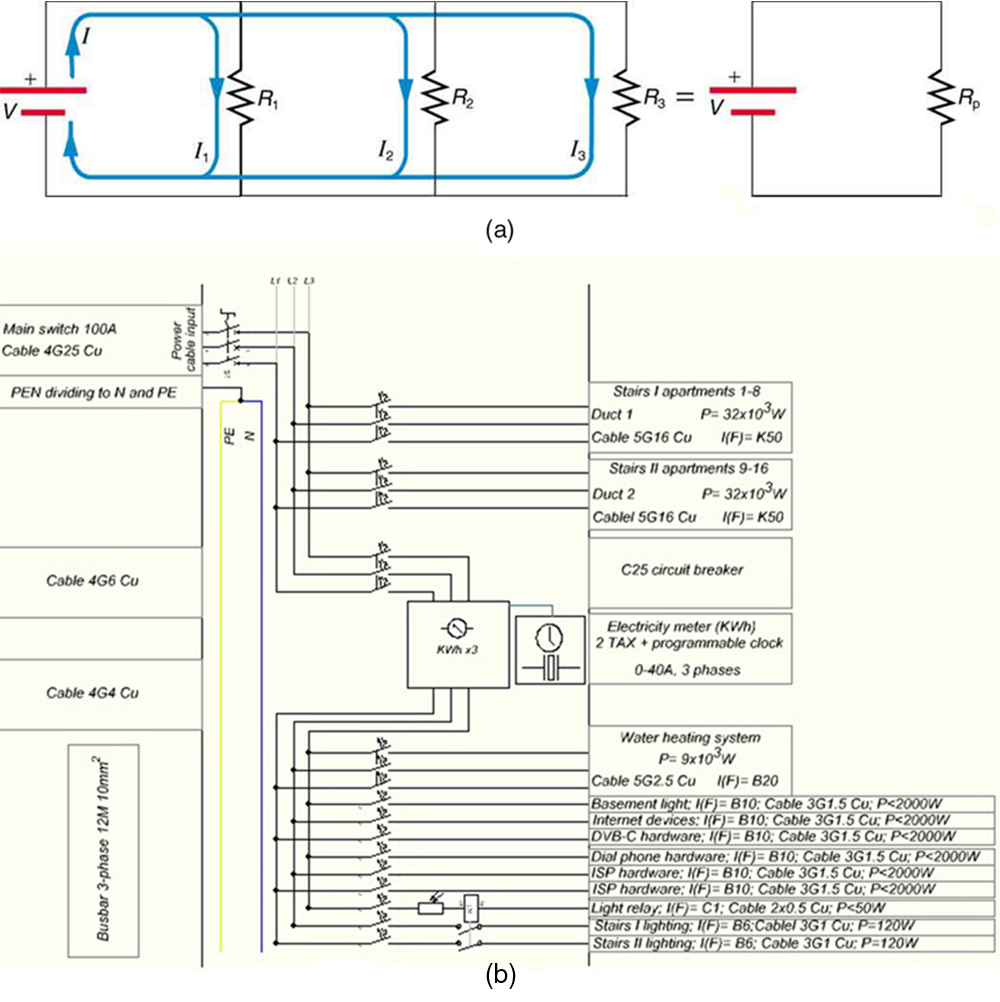
\includegraphics[width=0.45\textwidth,trim=0cm 13.5cm 5.5cm 0cm,clip=true]{parallel.jpeg}
\caption{\label{fig:para} \small A DC circuit with three resistors.}
\end{figure}
\begin{figure}
\centering
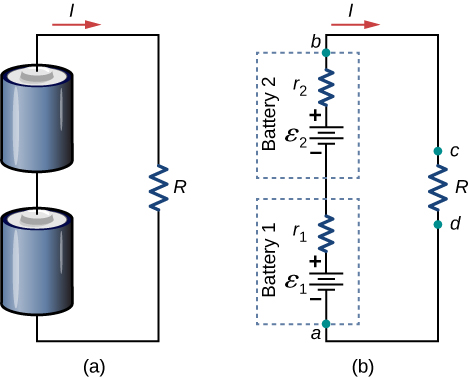
\includegraphics[width=0.15\textwidth,trim=0cm 0.5cm 4cm 0cm,clip=true]{series_batt.jpg}
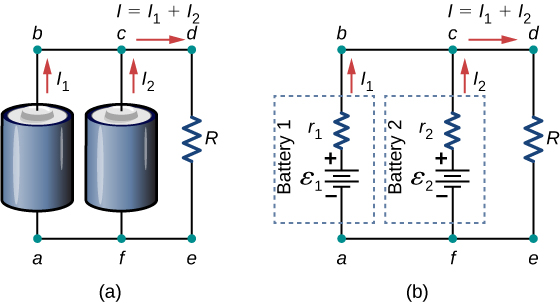
\includegraphics[width=0.2\textwidth,trim=0cm 0.5cm 5.5cm 0.41cm,clip=true]{parallel_batt.jpg}
\caption{\label{fig:batt} \small (Left) A DC circuit with two batteries in series, and a resistance $R = 0.5$ k$\Omega$. (Bottom) A DC circuit with two batteries in parallel, and a resistance $R = 0.5$ k$\Omega$.}
\end{figure}

\section{Unit 3: Magnetism I}
\begin{figure}
\centering
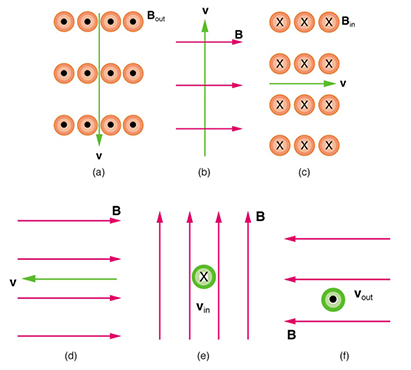
\includegraphics[width=0.49\textwidth,trim=0cm 2.8cm 0cm 0cm,clip=true]{Bfield.jpeg}
\caption{\label{fig:B} Three cases involving the particle velocity $\vec{v}$, and $\vec{B}$ field.}
\end{figure}
\noindent
\begin{enumerate}
\item Consider Fig. \ref{fig:B}. Fill in Tab. \ref{tab:ex} of directions below for the Lorentz force, assuming a \textbf{negatively charged} particle.  Let $\hat{i}$ represent right, $\hat{j}$ represent up, and $\hat{k}$ represent out of the page.
\begin{table}
\small
\centering
\begin{tabular}{| c | c | c | c |}
\hline
Case & v direction & B direction & F direction \\ \hline
(a) & down & out & right \\ \hline
(b) & up & right & out \\ \hline
(c) & right & in & down \\ \hline
\end{tabular}
\caption{\label{tab:ex} Table of directions for to Fig. \ref{fig:B}.}
\end{table}
\normalsize
\item An electron moving at $4.00\times 10^3$ m s$^{-1}$ in a 1.25-T magnetic field experiences a magnetic force of $1.40\times 10^{-16}$ N. What angle does the velocity of the electron make with the magnetic field? There are two possible answers. \\ \\
\textit{ $\theta = 10.08$ degrees.}
\item (a) An oxygen-16 ion with a mass of $2.66\times 10^{-26}$ kg travels at $5.00\times 10^6$ m/s perpendicular to a 1.20-T magnetic field, which makes it move in a circular arc with a 0.231-m radius. What positive charge is on the ion? (b) What is the ratio of this charge to that of the electron? (c) A mass spectrometer is being used to separate common oxygen-16 from the much rarer oxygen-18, taken from a sample of old glacial ice\footnote{The relative abundance of these oxygen isotopes is related to climatic temperature at the time the ice was deposited.}. The ratio of the masses of these two ions is 16 to 18.  For the same charge, what would the radius of the circular arc be for the oxygen-18?  \textit{Hint: scaling problem.} \\ \\
\textit{(a) $4.8 \times 10^{-19}$ C. (b) 3 (c) $(18/16)*0.231$ m, or 0.26 m.}
\end{enumerate}
\end{document}
